\documentclass[sigconf]{acmart}

% --- Packages ---
\usepackage{booktabs}
\usepackage{multirow}
\usepackage{amsmath,amsfonts}
\usepackage{tikz}
\usepackage{url}
\usepackage{xurl}
\usepackage{stfloats}
\usepackage{enumitem}

\emergencystretch=1.5em
\usetikzlibrary{shapes.geometric, arrows.meta, positioning, calc}

% Compact spacing for 5-page camera-ready format
\setlist[itemize]{nosep, leftmargin=1.1em, itemsep=1pt, topsep=2pt}
\setlist[enumerate]{nosep, leftmargin=1.2em, itemsep=1pt, topsep=2pt}
\setlength{\textfloatsep}{6pt plus 1.5pt minus 1.5pt}
\setlength{\dbltextfloatsep}{7pt plus 1.5pt minus 1.5pt}
\setlength{\abovecaptionskip}{3pt plus 1pt minus 1pt}
\setlength{\belowcaptionskip}{2pt plus 1pt minus 1pt}
\setlength{\abovedisplayskip}{4pt plus 1pt minus 1pt}
\setlength{\belowdisplayskip}{4pt plus 1pt minus 1pt}

% Suppress ACM Reference Format and Copyright block for clean conference submission
\settopmatter{printacmref=false}
\renewcommand\footnotetextcopyrightpermission[1]{}
\pagestyle{plain}

% ACM Rights & Conference Metadata for ICIIT 2027
\setcopyright{none}
\acmConference[ICIIT 2027]{2027 12th International Conference on Intelligent Information Technology}{March 04--07, 2027}{Ho Chi Minh City, Vietnam}
\acmYear{2027}
\copyrightyear{2027}
\acmDOI{}
\acmISBN{}

\begin{document}

\title[Benchmarking Inverse Reasoning and Tabular Transformation Discovery in Frontier LLMs]{Benchmarking Inverse Reasoning and Tabular Transformation Discovery in Frontier Large Language Models: A Two-Tier Autonomous Evaluation Harness}

\author{Viet Dao}
\affiliation{%
  \institution{FPT University}
  \city{Hanoi}
  \country{Vietnam}
}
\email{daothevietnb123@gmail.com}

\begin{abstract}
Reverse engineering the latent data-generating mechanisms of tabular datasets is a fundamental inverse problem that challenges inductive reasoning, feature discovery, and program synthesis. While Large Language Models (LLMs) excel at forward code generation, their ability to reconstruct hidden parametric pipelines solely from observational input-output tables remains underexplored. We introduce the \textbf{Tabular Transformation Discovery Harness}, an autonomous two-tier evaluation framework separating hypothesis search from code compilation across six structural complexity classes (from atomic unary operations to deep hybrid Abstract Syntax Trees, ASTs) spanning eight real-world domains ($N=48$ tasks). The harness enforces strict epistemic isolation: an agentic discovery phase inside a stateless Read-Eval-Print Loop (REPL) sandbox with adaptive budgets is decoupled from an independent evaluation phase on hidden holdout splits. Benchmarking two frontier agents (Claude 3.5 Sonnet, Gemini 2.0 Flash), a lightweight agent (GPT-4o mini), and an exhaustive depth-3 search lower bound across two evaluation seeds reveals distinct trade-offs: Claude 3.5 Sonnet achieves a $68.8 \pm 2.9\%$ submission rate with $0.829 \pm 0.025$ conditional ($0.569 \pm 0.007$ penalized) transformed accuracy, whereas Gemini 2.0 Flash attains $0.809 \pm 0.049$ conditional accuracy ($0.811 \pm 0.060$ Operator F1) but submits on only $50.0 \pm 0.0\%$ of tasks ($0.405 \pm 0.025$ penalized) due to conservative residual pursuit and premature unparsed terminations. A multi-model ablation shows that direct generation without REPL execution collapses transformed accuracy (0.024--0.050), whereas disclosing oracle operators unlocks 0.661--0.989 conditional synthesis accuracy ($\ge$0.993 Operator F1), indicating that hypothesis search under observational uncertainty—rather than code compilation—constitutes the primary bottleneck. Code and benchmark suites are available at \url{https://github.com/mini-smart-lab/tabular-transformation}.
\end{abstract}

\begin{CCSXML}
<ccs2012>
   <concept>
       <concept_id>10010147.10010257</concept_id>
       <concept_desc>Computing methodologies~Machine learning</concept_desc>
       <concept_significance>500</concept_significance>
   </concept>
   <concept>
       <concept_id>10010147.10010178.10010187</concept_id>
       <concept_desc>Knowledge representation and reasoning</concept_desc>
       <concept_significance>500</concept_significance>
   </concept>
</ccs2012>
\end{CCSXML}

\ccsdesc[500]{Computing methodologies~Machine learning; Knowledge representation and reasoning}
\keywords{Tabular Data, Inverse Program Induction, Autonomous Agent, Two-Tier Evaluation Harness, Symbolic Recovery}

\maketitle

\section{Introduction}
Tabular data remains the predominant modality in industrial, scientific, and financial domains~\cite{borisov2022deep,grinsztajn2022tree}, yet presents permutation-invariant columns, heterogeneous distributions, and non-linear cross-column dependencies that challenge autoregressive LLMs~\cite{sui2024table}. A central problem at the intersection of automated machine learning and program synthesis is \emph{inverse tabular transformation reasoning}: given observational tables $\mathcal{D}_{\text{before}}$ and $\mathcal{D}_{\text{after}}$, can an autonomous agent infer and synthesize the latent transformation $\mathcal{T}$ such that $\mathcal{T}(\mathcal{D}_{\text{before}}) \approx \mathcal{D}_{\text{after}}$? This capability underpins auditing undocumented ETL (Extract, Transform, Load) pipelines, scientific equation recovery~\cite{schmidt2009distilling,udrescu2020ai}, and privacy leakage auditing in synthetic data~\cite{stadler2022synthetic}.

Unlike forward benchmarks such as HumanEval~\cite{chen2021evaluating} and SWE-bench~\cite{jimenez2024swebench}, inverse tabular induction requires scientific hypothesis formation in a Read-Eval-Print Loop (REPL) sandbox: inspecting multivariate numeric distributions, disentangling candidate laws via interactive execution, and compiling a self-contained parametric $\texttt{transform}(\texttt{df})$ function that generalizes out-of-distribution. Prior evaluations suffer from three flaws: reliance on toy synthetic distributions rather than collinear empirical tables, shared train/test execution environments risking leakage, and metrics conflating code synthesis with hypothesis search.

We introduce the \textbf{Tabular Transformation Discovery Harness} (Figure~\ref{fig:two_tier_arch}), contributing: (1) a \textbf{6-class Abstract Syntax Tree (AST) complexity taxonomy} scaling from atomic unary operations (Class 0) to deep hybrid Directed Acyclic Graphs (DAGs) with piecewise conditionals (Class 5); (2) a \textbf{two-tier epistemic isolation architecture} separating Tier-1 stateless REPL discovery (under class-adaptive budgets) from air-gapped Tier-2 evaluation on unseen holdouts; (3) a \textbf{balanced 48-task benchmark} spanning 8 UCI/OpenML domains ($8 \times 6 = 48$); (4) a \textbf{two-seed empirical comparison} across Claude 3.5 Sonnet, Gemini 2.0 Flash, GPT-4o mini, and an exhaustive depth-3 lower bound; and (5) a \textbf{three-mode multi-model ablation} isolating REPL feedback and oracle operator knowledge.

\begin{figure*}[t!]
\centering
\resizebox{0.96\textwidth}{!}{
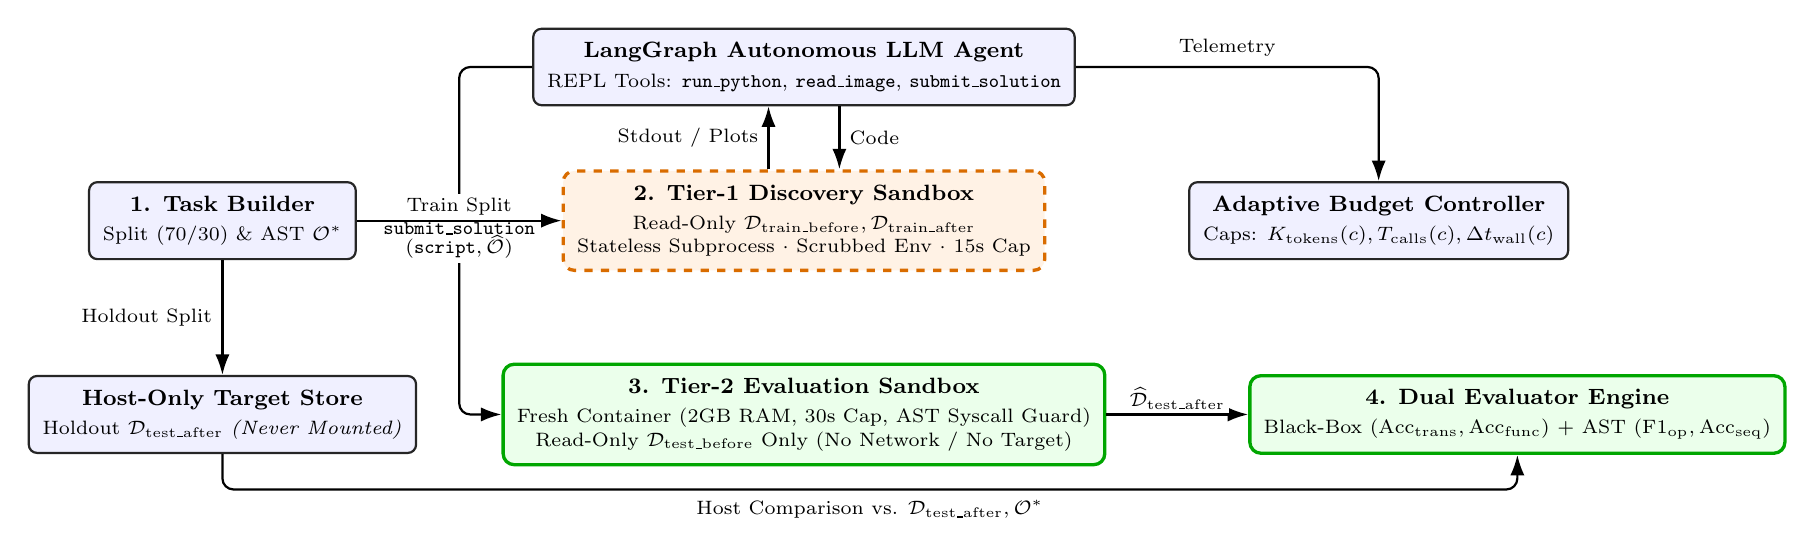
\begin{tikzpicture}[
    node distance=1.0cm and 1.6cm,
    box/.style={rectangle, draw=black!85, fill=blue!6, rounded corners=3pt, thick, align=center, inner sep=5pt, font=\footnotesize},
    sand/.style={rectangle, draw=orange!85!black, fill=orange!10, rounded corners=4pt, dashed, very thick, align=center, inner sep=5pt, font=\footnotesize},
    eval/.style={rectangle, draw=green!65!black, fill=green!8, rounded corners=4pt, very thick, align=center, inner sep=5pt, font=\footnotesize},
    arrow/.style={-{Latex[length=2.6mm, width=1.8mm]}, thick}
]
\node[box] (taskgen) {\textbf{1. Task Builder}\\[1pt]\scriptsize Split (70/30) \& AST $\mathcal{O}^*$};
\node[sand, right=2.6cm of taskgen] (sand1) {\textbf{2. Tier-1 Discovery Sandbox}\\[1pt]\scriptsize Read-Only $\mathcal{D}_{\text{train\_before}}, \mathcal{D}_{\text{train\_after}}$\\[-1pt]\scriptsize Stateless Subprocess $\cdot$ Scrubbed Env $\cdot$ 15s Cap};
\node[box, above=0.8cm of sand1] (agent) {\textbf{LangGraph Autonomous LLM Agent}\\[1pt]\scriptsize REPL Tools: \texttt{run\_python}, \texttt{read\_image}, \texttt{submit\_solution}};
\node[box, right=1.8cm of sand1] (budget) {\textbf{Adaptive Budget Controller}\\[1pt]\scriptsize Caps: $K_{\text{tokens}}(c), T_{\text{calls}}(c), \Delta t_{\text{wall}}(c)$};

\node[eval, below=1.15cm of sand1] (sand2) {\textbf{3. Tier-2 Evaluation Sandbox}\\[1pt]\scriptsize Fresh Container (2GB RAM, 30s Cap, AST Syscall Guard)\\[-1pt]\scriptsize Read-Only $\mathcal{D}_{\text{test\_before}}$ Only (No Network / No Target)};
\node[eval, right=1.8cm of sand2] (evaluator) {\textbf{4. Dual Evaluator Engine}\\[1pt]\scriptsize Black-Box ($\text{Acc}_{\text{trans}}, \text{Acc}_{\text{func}}$) + AST ($\text{F1}_{\text{op}}, \text{Acc}_{\text{seq}}$)};
\node[box] (hiddendata) at (taskgen |- sand2) {\textbf{Host-Only Target Store}\\[1pt]\scriptsize Holdout $\mathcal{D}_{\text{test\_after}}$ \emph{(Never Mounted)}};

\draw[arrow] (taskgen) -- node[left, font=\scriptsize]{Holdout Split} (hiddendata);
\draw[arrow] ([xshift=0.45cm]agent.south) -- node[right, font=\scriptsize]{Code} ([xshift=0.45cm]sand1.north);
\draw[arrow] ([xshift=-0.45cm]sand1.north) -- node[left, font=\scriptsize]{Stdout / Plots} ([xshift=-0.45cm]agent.south);
\draw[arrow, rounded corners=4pt] (agent.east) -| node[pos=0.25, above, font=\scriptsize]{Telemetry} (budget.north);
\path (taskgen.east) -- (sand1.west) coordinate[midway] (midgap);
\draw[arrow, rounded corners=4pt] (agent.west) -- (midgap |- agent.west) -- node[fill=white, align=center, font=\scriptsize, inner sep=1.5pt]{$\texttt{submit\_solution}$\\[-1pt]$(\texttt{script}, \widehat{\mathcal{O}})$} (midgap |- sand2.west) -- (sand2.west);
\draw[arrow] (taskgen) -- node[above, fill=white, inner sep=1.5pt, font=\scriptsize]{Train Split} (sand1);
\draw[arrow] (sand2) -- node[above, fill=white, inner sep=1.5pt, font=\scriptsize]{$\widehat{\mathcal{D}}_{\text{test\_after}}$} (evaluator);
\path (hiddendata.south) -- ++(0, -0.45) coordinate (bot);
\draw[arrow, rounded corners=4pt] (hiddendata.south) -- (hiddendata.south |- bot) -- node[below, font=\scriptsize]{Host Comparison vs. $\mathcal{D}_{\text{test\_after}}, \mathcal{O}^*$} (evaluator.south |- bot) -- (evaluator.south);
\end{tikzpicture}
}
\caption{Two-Tier Tabular Transformation Discovery Harness. \textbf{(1) Task Builder} creates 70/30 splits and AST $\mathcal{O}^*$. \textbf{(2) Tier-1 Sandbox} isolates exploratory Python execution and plots on training tables under adaptive budgets. \textbf{(3) Tier-2 Sandbox} evaluates \texttt{transform(df)} in an air-gapped container seeing only $\mathcal{D}_{\text{test\_before}}$. \textbf{(4) Dual Evaluator} scores predictions and parsed ASTs against host-isolated ground truth.}
\label{fig:two_tier_arch}
\end{figure*}

\section{Related Work}
\noindent\textbf{Tabular LLMs and Foundation Models:} Recent work adapts foundation models to tabular data via serialization (TabLLM~\cite{hegselmann2023tabllm}), instruction tuning (Table-GPT~\cite{li2024tablegpt}), structural table benchmarks~\cite{sui2024table}, and two-stage in-context attention (TabICL~\cite{qu2025tabicl}). All operate in the forward predictive or question-answering (QA) regime without an execution sandbox, whereas we study inverse programmatic pipeline induction from input-output table pairs.

\noindent\textbf{Program Synthesis, Symbolic Regression, and Agents:} Programming-by-Example (PBE) wrangling tools (FlashFill~\cite{gulwani2011flashfill}, Foofah~\cite{jin2017foofah}, Auto-Pipeline~\cite{yang2021autopipeline}) target discrete relational/string edits rather than continuous numerical compositions. Evolutionary symbolic regression (genetic programming~\cite{schmidt2009distilling}, AI Feynman~\cite{udrescu2020ai}, PySR~\cite{cranmer2023pysr}) and LLM equation discovery (LLM-SR~\cite{shojaee2025llmsr}, LLM-SRBench~\cite{shojaee2025llmsrbench}) optimize analytical expressions for an isolated target with pre-identified inputs using evolutionary population search and continuous parameter optimizers (e.g., BFGS). In contrast, our harness evaluates autonomous multi-turn ReAct/REPL agents~\cite{yao2023react,langgraph2024}—distinguishing it from natural-language-prompted forward coding benchmarks (DS-1000~\cite{lai2023ds1000}, DA-Code~\cite{huang2024dacode}, FeatEng~\cite{pietruszka2025feateng})—under three distinct tabular challenges: (i) while detecting changed target columns in $\mathcal{C}_{\text{after}}$ is trivial via residual checking ($\|\mathcal{D}_{\text{train\_after}}[:, c] - \mathcal{D}_{\text{train\_before}}[:, c]\| > \epsilon$), the core challenge is \emph{identifying latent source predictor columns} in $\mathcal{D}_{\text{before}}$ when interaction targets are anonymized or overwritten (Classes 3--5); (ii) \emph{AST-level operator normalization} of stateful scalers ($\Omega_3$, distinguishing $\text{StandardScaler}$ from generic affine coefficients $ax+b$) frozen strictly on training splits; and (iii) discontinuous piecewise thresholds ($\Omega_5$).

\section{Problem Formulation and Harness Design}
\subsection{Formalization and 24-Operator Vocabulary}
Given an observational table $\mathcal{D}_{\text{before}} = \{\mathbf{x}^{(i)}\}_{i=1}^N \in \mathbb{R}^{N \times M}$ with schema $\mathcal{C}_{\text{before}}$, a deterministic parameterized pipeline $\mathcal{T}: \mathbb{R}^M \to \mathbb{R}^P$ produces $\mathcal{D}_{\text{after}} = \mathcal{T}(\mathcal{D}_{\text{before}}) \in \mathbb{R}^{N \times P}$ with schema $\mathcal{C}_{\text{after}}$. In-place transformed columns retain their identifiers, while synthesized/overwritten interaction targets adopt neutral identifiers so column names leak no dependencies. $\mathcal{T}$ forms an AST over 24 canonical operators $\Omega = \bigcup_{k=1}^5 \Omega_k$: \textbf{(1) Power \& Unary ($\Omega_1$, 8 ops):} $\text{Square}$ ($x^2$), $\text{SquareRoot}$ ($\sqrt{x}$), $\text{Cube}$ ($x^3$), $\text{CubeRoot}$ ($\sqrt[3]{x}$), $\text{Exp}$ ($e^x$), $\text{Log}$ ($\ln x$), $\text{Log1p}$ ($\ln(x+1)$), $\text{Inverse}$ ($1/x$); \textbf{(2) Trig/Activation ($\Omega_2$, 5 ops):} $\text{Sin}$, $\text{Cos}$, $\text{Tanh}$, $\text{Sigmoid}$, $\text{Abs}$; \textbf{(3) Stateful Scalers ($\Omega_3$, 2 ops):} $\text{StandardScaler}$ ($(x-\mu)/\sigma$), $\text{MinMaxScaler}$ ($(x-x_{\min})/(x_{\max}-x_{\min})$); \textbf{(4) Bivariate Interactions ($\Omega_4$, 4 ops):} $\text{Add}$, $\text{Subtract}$, $\text{Multiply}$, $\text{Divide}$; \textbf{(5) Piecewise Logic ($\Omega_5$, 5 ops):} $\text{IndicatorZero}$ ($\mathbf{1}_{\{x>0\}}$), $\text{IndicatorMean}$ ($\mathbf{1}_{\{x>\mu\}}$), $\text{ClipZero}$ ($\max(0,x)$), $\text{PiecewiseLog}$ ($\mathbf{1}_{\{x>0\}}\ln x$), and $\text{ConditionalInteraction}$ ($\mathbf{1}_{\{x_j>\theta\}}\cdot x_i$).

\noindent\textbf{Stateful Scalers \& Data Splitting:} Moments for $\Omega_3$ and $\text{IndicatorMean}$ ($\mu$, population std $\sigma$ with $\text{ddof}=0$ matching \texttt{numpy} and \texttt{scikit-learn} defaults relative to $\epsilon=10^{-4}$, $x_{\min}$, $x_{\max}$) are fitted strictly on $\mathcal{D}_{\text{train\_before}}$ and embedded as hardcoded floating-point literals in \texttt{transform(df)}, preventing test-set leakage. Each dataset is partitioned into observed $\mathcal{D}_{\text{train}}$ (70\%) and hidden $\mathcal{D}_{\text{test}}$ (30\%) via uniform permutation with a fixed benchmark generation seed ($\text{seed}_{\text{split}}=42$), ensuring $\mathcal{D}_{\text{train}} \cap \mathcal{D}_{\text{test}} = \emptyset$. Given $\mathcal{D}_{\text{train}}$ only, the agent must synthesize $\widehat{\mathcal{T}}$ maximizing column recovery on $\mathcal{D}_{\text{test}}$ while recovering $\mathcal{O}^* \subseteq \Omega$. Averaging across all $c \in \mathcal{C}_{\text{after}}$ defines \textbf{Functional Column Accuracy} ($\text{Acc}_{\text{func}}$), whereas our primary metric \textbf{Transformed Column Accuracy} ($\text{Acc}_{\text{trans}}$, Eq.~\ref{eq:acc_trans}) restricts evaluation to genuinely altered columns $\mathcal{C}_{\text{trans}} \subseteq \mathcal{C}_{\text{after}}$, eliminating the identity baseline floor $(|\mathcal{C}_{\text{after}}| - |\mathcal{C}_{\text{trans}}|)/|\mathcal{C}_{\text{after}}|$ conferred by unchanged columns.

\subsection{Six Structural Complexity Classes (C0--C5)}
We define six structural classes via transformed column count $|\mathcal{C}_{\text{trans}}|$ and AST depth $d$:
\begin{itemize}
    \item \textbf{C0 (Atomic Unary):} $|\mathcal{C}_{\text{trans}}|=1$ column, $y=f(x)$ ($d=1$).
    \item \textbf{C1 (Independent Unary):} $|\mathcal{C}_{\text{trans}}|=2$ columns, $y_j=f_j(x_j)$ ($d=1$).
    \item \textbf{C2 (Composed Chains):} $|\mathcal{C}_{\text{trans}}|=3$ columns, $y_j=f_{j,2}(f_{j,1}(x_j))$ ($d=2$). For depth $d \ge 2$, domain constraints and scaler moments ($\mu,\sigma,x_{\min},x_{\max}$) for $f_{j,2}$ are fitted on intermediate values $f_{j,1}(x_j)$ over $\mathcal{D}_{\text{train}}$.
    \item \textbf{C3 (Multi-Column Interactions):} $|\mathcal{C}_{\text{trans}}|=4$: 3 unary chains ($d=2$) plus 1 bivariate interaction $z = x_i \star x_j$ ($\star \in \{+,-,\times,\div\}$).
    \item \textbf{C4 (Piecewise / Conditional):} $|\mathcal{C}_{\text{trans}}|=4$: 3 chains ($d=2$) prioritizing unary $g \in \Omega_5$, plus $z = \mathbf{1}_{\{x_j > \theta\}}\cdot x_i$ with threshold $\theta \in \{0, \mu\}$ ($\mu$ fitted on $\mathcal{D}_{\text{train\_before}}$), where $g(x) = h(x)$ if $x>\theta$ else $0$ for $h(x) \in \{1, x, \ln x\}$ (yielding $f_{j,2}(0)$ on inactive composed branches). \texttt{PiecewiseLog} uses \texttt{np.where(x > 0, np.log(np.maximum(x, 1e-12)), 0.0)}.
    \item \textbf{C5 (Deep Hybrid AST):} Up to $|\mathcal{C}_{\text{trans}}| \le 6$ columns forming DAGs up to $d=3$ with multiple interactions and outer unary compositions ($y=f(x_i \star x_j)$). On low-dimensional tables (e.g., \textsf{banknote\_authentication}, $M=4$), the generator clamps counts to respect non-overlapping targets, yielding $|\mathcal{C}_{\text{trans}}|=2$ in C5.
\end{itemize}
All branches read concurrently from an immutable snapshot of $\mathcal{D}_{\text{before}}$ and overwrite designated targets in-place ($P=M$).

\subsection{Two-Tier Isolation and Evaluation Metrics}
\label{sec:metrics}
In \textbf{Tier 1}, the agent explores read-only $\mathcal{D}_{\text{train}}$ via three tools: \texttt{run\_python(code)} (fresh subprocess, stripped \texttt{API\_KEY}/\texttt{TOKEN}, 15s timeout, stateless RAM across calls), \texttt{read\_image(path)} (visual chart inspection), and \texttt{submit\_solution(script, $\widehat{\mathcal{O}}$)}. Episodes enforce class-adaptive caps for $c \in \{0,\dots,5\}$: $T_{\text{calls}}(c) \in (8,10,14,18,24,30)$, $K_{\text{tokens}}(c) \in (60,80,120,160,220,300)\text{k}$, and $\Delta t_{\text{wall}}(c) \in (120,120,180,240,300,360)\text{s}$. In \textbf{Tier 2}, submitted scripts pass an AST syscall guard (blocking \texttt{subprocess}, sockets, filesystem writes) and execute in an isolated container (2GB RAM, 30s timeout, no network) mounting only $\mathcal{D}_{\text{test\_before}}$; $\mathcal{D}_{\text{test\_after}}$ remains host-only.

\noindent\textbf{Black-Box Functional Metrics:} Column match over $N_{\text{test}}$ rows and transformed accuracy are defined as:
\begin{align}
m(c) &= \frac{1}{N_{\text{test}}}\sum_{i=1}^{N_{\text{test}}} \mathbf{1}_{\{|\widehat{D}_{i,c}-D_{i,c}| < \epsilon\cdot(|D_{i,c}|+1)\}}, \label{eq:col_match}\\
\text{Acc}_{\text{trans}} &= \frac{1}{|\mathcal{C}_{\text{trans}}|} \sum_{c\in\mathcal{C}_{\text{trans}}} \mathbf{1}_{\{m(c)\ge 0.99\}}, \label{eq:acc_trans}
\end{align}
with $\epsilon=10^{-4}$ (0 for missing/non-finite columns); $\text{Acc}_{\text{func}}$ averages over all $c \in \mathcal{C}_{\text{after}}$. To avoid inflated reporting, \textbf{Conditional Accuracy} ($\text{Acc}_{\text{cond}} = \frac{1}{N_{\text{sub}}}\sum_{i:\text{sub}_i}\text{Acc}_i$) scores submitted episodes, whereas \textbf{Penalized Accuracy} ($\text{Acc}_{\text{pen}} = \frac{1}{N_{\text{total}}}\sum_{i=1}^{N_{\text{total}}}\mathbf{1}_{\{\text{sub}_i\}}\text{Acc}_i$) assigns 0 to non-submissions ($\text{Acc}_{\text{pen}} = \text{Sub.\ Rate} \times \text{Acc}_{\text{cond}}$ per individual run).

\noindent\textbf{White-Box Symbolic Metrics:} Python's \texttt{ast} extracts executed operators $\widehat{\mathcal{O}}_{\text{AST}}$ as evaluation ground. \textbf{Operator F1} ($\text{F1}_{\text{op}}$) computes harmonic mean of multiset precision ($|\widehat{\mathcal{O}}_{\text{AST}}\cap\mathcal{O}^*|/|\widehat{\mathcal{O}}_{\text{AST}}|$, 0 if empty) and recall ($|\widehat{\mathcal{O}}_{\text{AST}}\cap\mathcal{O}^*|/|\mathcal{O}^*|$) using multiset intersection $|\widehat{\mathcal{O}}_{\text{AST}}\cap\mathcal{O}^*| = \sum_{\omega\in\Omega}\min(\text{count}_{\widehat{\mathcal{O}}_{\text{AST}}}(\omega), \text{count}_{\mathcal{O}^*}(\omega))$. \textbf{Exact Sequence Accuracy} ($\text{Acc}_{\text{seq}}$) checks column-level depth-first topological sequence match (sorting commutative $\text{Add}$/$\text{Multiply}$ operands alphabetically). Canonical AST normalization resolves numpy/pandas equivalents, but static AST patterns cannot disambiguate semantic intent—e.g., \texttt{(df[c]-a)/b} as $\text{StandardScaler}$ ($\Omega_3$) vs.\ $\text{Subtract}$+$\text{Divide}$ ($\Omega_4$) without data tracing—necessitating paired black-box evaluation.

\section{Experimental Setup}
\label{sec:exp_setup}
\noindent\textbf{Benchmark Tasks ($N=48$):} We compile a balanced full-factorial suite ($8 \text{ datasets} \times 6 \text{ classes} = 48$ tasks; $n=8$/class, $n=6$/domain) from UCI~\cite{dua2019uci} and OpenML~\cite{vanschoren2014openml}: \textsf{airfoil\_self\_noise} ($N=1,503$, $N_{\text{train}}=1,052$, $N_{\text{test}}=451$, all $M=6$ attributes), \textsf{diabetes} ($768/537/231$, $M=8$), \textsf{concrete\_strength} ($1,030/721/309$, $M=8$), \textsf{cpu\_small} ($8,192/5,734/2,458$, $M=12$), \textsf{wine\_quality} ($1,599/1,119/480$, $M=11$), \textsf{breast\_cancer} ($569/398/171$, $M=30$), \textsf{california\_housing} ($20,640/14,448/6,192$, $M=8$), and \textsf{banknote\_authentication} ($1,372/960/412$, $M=4$). Because per-class and per-domain subsets contain 8 and 6 tasks respectively, fine-grained subset comparisons carry modest statistical power and should be interpreted with caution. Tasks use a fixed generation seed ($\text{seed}_{\text{split}}=42$) and \emph{raw-data rejection sampling}: operators are eligible only if raw distributions satisfy domain bounds without clipping (restricting negative bimodal columns in \textsf{banknote\_authentication} to $\text{Square}$, $\text{Cube}$, $\text{CubeRoot}$, $\text{Sin}$, $\text{Tanh}$, $\text{StandardScaler}$, $\Omega_4$, and $\Omega_5$ ops like $\text{IndicatorZero}$, $\text{IndicatorMean}$, $\text{ClipZero}$).

\noindent\textbf{Models, Proxy, and Multi-Seed Protocol:} We evaluate two frontier agents—\textbf{Claude 3.5 Sonnet} (\path{claude-3-5-sonnet-20241022}~\cite{anthropic2024claude35}) and \textbf{Gemini 2.0 Flash} (\path{gemini-2.0-flash-exp}~\cite{geminiteam2025gemini}, with thinking trace)—and one lightweight agent, \textbf{GPT-4o mini} (\path{gpt-4o-mini-2024-07-18}~\cite{openai2024gpt4o}). All three LLMs are natively multimodal, orchestrated within the same LangGraph state-machine workflow~\cite{langgraph2024} with identical tool access (\texttt{run\_python}, \texttt{read\_image}, \texttt{submit\_solution}), and queried through the Kaggle-provided API proxy (ensuring host credential scrubbing, rate-limit backoff, uniform token auditing including thinking tokens, and latency homogenization). A non-LLM \textbf{Symbolic Enumeration} baseline is formulated strictly as a stateless algebraic expression search—an unguided depth-3 exhaustive lower bound via $L_1$ residual minimization that evaluates candidate operators on training data but emits dynamic DataFrame moment calls (e.g., \texttt{df[c].mean()}) rather than freezing training-split scalar literals ($\mu,\sigma,x_{\min},x_{\max},\theta$) across splits. All LLMs run at $T=0.0$ across two evaluation seeds ($\text{seed}\in\{42,43\}$, $S=2$, bounded by proxy compute quota), capturing two-run trajectory stability over the fixed 48-task suite.

\noindent\textbf{Three-Mode Ablation ($\text{seed}=42$):} (1) \textbf{Direct Symbolic Gen.\ (No Tools)}: \texttt{run\_python}/\texttt{read\_image} are removed from API tool registration; unparsed responses terminate immediately without retry (Claude and GPT-4o mini submit fallback scripts on 48/48 tasks; Gemini submits 15/48 = 31.2\% due to premature termination without tool dispatch); (2) \textbf{Standard Full Agent}; (3) \textbf{Oracle Operators Revealed}: $\mathcal{O}^*$ names given in prompt (Claude and GPT-4o mini 48/48, Gemini 37/48 = 77.1\%).

\section{Empirical Results and Analysis}
\begin{table*}[t]
\centering
\caption{Two-Seed Benchmark Comparison ($N=48$ Tasks across 8 Domains $\times$ 6 Classes; $\text{Mean}\pm\text{Std}$ over $S=2$ seeds $\text{seed}\in\{42,43\}$ at $T=0.0$ capturing trajectory stability; deterministic single run for Symbolic Enumeration). Both aggregate metrics and per-class Penalized Transformed Accuracy ($\text{Acc}_{\text{pen}}$, $n=8$ tasks/class)\textsuperscript{a} are reported. Best overall is bolded; best LLM is underlined.}
\label{tab:main_and_class}
\resizebox{\textwidth}{!}{%
\begin{tabular}{ll ccccc cccccc}
\toprule
\multirow{2}{*}{\textbf{Model}} & \multirow{2}{*}{\textbf{Paradigm}} & \multicolumn{5}{c}{\textbf{Aggregate Suite Metrics ($N=48$)}} & \multicolumn{6}{c}{\textbf{Per-Class $\text{Acc}_{\text{pen}}$ ($n=8$ per class)\textsuperscript{a}}} \\
\cmidrule(lr){3-7} \cmidrule(lr){8-13}
 & & \textbf{Sub.\ Rate} & \textbf{Trans.\ (Cond)} & \textbf{Trans.\ (Pen)} & \textbf{Func.\ (Pen / Cond)} & \textbf{Op.\ F1} & \textbf{C0} & \textbf{C1} & \textbf{C2} & \textbf{C3} & \textbf{C4} & \textbf{C5} \\
\midrule
Claude 3.5 Sonnet & Frontier Agent & $68.8 \pm 2.9\%$ & \textbf{\underline{$0.829 \pm 0.025$}} & \underline{$0.569 \pm 0.007$} & $0.641 \pm 0.037$ ($0.932$) & $0.736 \pm 0.021$ & \textbf{\underline{$.875\pm.000$}} & \textbf{\underline{$.938\pm.088$}} & $.312\pm.147$ & \underline{$.438\pm.088$} & \underline{$.500\pm.044$} & \underline{$.354\pm.059$} \\
Gemini 2.0 Flash & Frontier Agent & $50.0 \pm 0.0\%$ & $0.809 \pm 0.049$ & $0.405 \pm 0.025$ & $0.453 \pm 0.021$ ($0.906$) & \underline{$0.811 \pm 0.060$} & $.750\pm.000$ & $.438\pm.088$ & $.229\pm.206$ & $.406\pm.088$ & $.344\pm.044$ & $.260\pm.103$ \\
GPT-4o mini & Lightweight Agent & \textbf{\underline{$100.0 \pm 0.0\%$}} & $0.485 \pm 0.018$ & $0.485 \pm 0.018$ & \underline{$0.799 \pm 0.011$ ($0.799$)} & $0.445 \pm 0.038$ & $.812\pm.088$ & $.750\pm.088$ & \underline{$.417\pm.059$} & $.391\pm.066$ & $.312\pm.133$ & $.229\pm.059$ \\
Symbolic Enum. & Exhaustive Lower Bound & \textbf{100.0\%} & 0.653 & \textbf{0.653} & \textbf{0.876 (0.876)} & \textbf{0.872} & .750 & .750 & \textbf{.667} & \textbf{.562} & \textbf{.812} & \textbf{.375} \\
\bottomrule
\end{tabular}%
}
\par\vspace{1pt}
{\scriptsize \textsuperscript{a} Because each complexity class C0--C5 contains $n=8$ tasks (one per domain), fine-grained class differences have limited statistical power and should be interpreted with caution.}
\end{table*}

\begin{table*}[t]
\centering
\caption{Reference-Seed Telemetry ($\text{seed}=42$, $N=48$): Termination Breakdown (Submitted, Token/Call Exceeded, Premature Stop), Mean Cumulative Tokens (including thinking traces), Mean Tool Calls (where Total includes initial and retried/rejected \texttt{submit\_solution} calls: 41/34 accepted for Claude, 25/24 Gemini, 51/48 GPT-4o mini), and Episode Wall / Sandbox Execution Time.}
\label{tab:telemetry_breakdown}
\resizebox{\textwidth}{!}{%
\begin{tabular}{l c c cccc ccc ccc cc}
\toprule
\textbf{Model Agent} & \textbf{$N$} & \textbf{Sub.\ Rate} & \textbf{Sub.} & \textbf{Tok.\ Ex.} & \textbf{Call Ex.} & \textbf{Stop} & \textbf{Tot.\ Tok.} & \textbf{In.\ Tok.} & \textbf{Out.\ Tok.} & \textbf{Tot.\ Calls} & \textbf{\texttt{python}} & \textbf{\texttt{image}} & \textbf{Wall (s)} & \textbf{Exec (s)} \\
\midrule
Claude 3.5 Sonnet & 48 & 70.8\% & 34 & 11 & 3 & 0 & 133,117 & 127,247 & 5,871 & 13.9 & 12.5 & 0.4 & 85.2 & 20.4 \\
Gemini 2.0 Flash & 48 & 50.0\% & 24 & 6 & 4 & 14 & 122,121 & 112,665 & 9,457 & 13.4 & 12.0 & 0.6 & 80.9 & 26.6 \\
GPT-4o mini & 48 & 100.0\% & 48 & 0 & 0 & 0 & 65,171 & 62,060 & 3,111 & 12.6 & 11.6 & 0.0 & 58.1 & 23.0 \\
\bottomrule
\end{tabular}%
}
\end{table*}

\begin{table*}[b!]
\centering
\caption{Three-Mode Ablation Study across Models ($N=48$, reference $\text{seed}=42$). In the No Tools mode, non-zero transformed accuracy (0.024--0.050) is an artifact of identity-preserving operations ($f(x)\equiv x$) on discrete features submitted via fallback \texttt{df.copy()}, yielding $\widehat{\mathcal{O}}=\emptyset$ ($\text{Op.\ F1}=0.000$).}
\label{tab:ablation_study}
\resizebox{\textwidth}{!}{%
\begin{tabular}{llcccccc}
\toprule
\textbf{Model} & \textbf{Ablation Condition} & \textbf{Submissions} & \textbf{Trans.\ (Cond)} & \textbf{Trans.\ (Pen)} & \textbf{Func.\ (Cond / Pen)} & \textbf{Op.\ F1 (Cond)} & \textbf{Seq.\ (Cond)} \\
\midrule
\textbf{Claude 3.5 Sonnet} & Direct Symbolic Gen.\ (No Tools) & 48/48 (100.0\%) & 0.024 & 0.024 & 0.679 (0.679) & 0.000 & 0.000 \\
 & Standard Interactive Discovery (Full) & 34/48 (70.8\%) & 0.811 & 0.575 & 0.942 (0.667) & 0.721 & 0.580 \\
 & Oracle Operators Revealed & 48/48 (100.0\%) & 0.943 & 0.943 & 0.974 (0.974) & 1.000 & 0.993 \\
\midrule
\textbf{Gemini 2.0 Flash} & Direct Symbolic Gen.\ (No Tools) & 15/48 (31.2\%) & 0.050 & 0.016 & 0.635 (0.198) & 0.000 & 0.000 \\
 & Standard Interactive Discovery (Full) & 24/48 (50.0\%) & 0.844 & 0.422 & 0.936 (0.468) & 0.853 & 0.736 \\
 & Oracle Operators Revealed & 37/48 (77.1\%) & 0.989 & 0.762 & 0.976 (0.752) & 1.000 & 1.000 \\
\midrule
\textbf{GPT-4o mini} & Direct Symbolic Gen.\ (No Tools) & 48/48 (100.0\%) & 0.024 & 0.024 & 0.679 (0.679) & 0.000 & 0.000 \\
 & Standard Interactive Discovery (Full) & 48/48 (100.0\%) & 0.472 & 0.472 & 0.807 (0.807) & 0.418 & 0.322 \\
 & Oracle Operators Revealed & 48/48 (100.0\%) & 0.661 & 0.661 & 0.868 (0.868) & 0.993 & 0.977 \\
\bottomrule
\end{tabular}%
}
\end{table*}

\subsection{Cross-Model and Exhaustive Baseline Comparison}
Table~\ref{tab:main_and_class} summarizes two-seed aggregate and per-class ($n=8$/class) results over the 48 tasks. Because per-class subsets contain 8 tasks each, class-level trends should be interpreted cautiously:
\begin{itemize}
    \item \textbf{Claude 3.5 Sonnet} achieves the highest conditional ($0.829 \pm 0.025$) and LLM penalized ($0.569 \pm 0.007$) transformed accuracy with a $68.8 \pm 2.9\%$ submission rate ($33.0/48$), solving shallow unary classes reliably ($0.875\pm 0.000$ C0, $0.938\pm 0.088$ C1) and retaining $62.5 \pm 17.7\%$ submission ($0.576 \pm 0.069$ cond., $0.354 \pm 0.059$ pen.) on Class 5 hybrid ASTs.
    \item \textbf{Gemini 2.0 Flash} attains the highest LLM Operator F1 ($0.811 \pm 0.060$) alongside $0.809 \pm 0.049$ conditional transformed accuracy, but submits on only $50.0 \pm 0.0\%$ ($24/48$; $0.405 \pm 0.025$ pen.) due to two factors: tight residual pursuit exhausting budgets when $\|\widehat{\mathcal{D}}-\mathcal{D}\|_\infty \ge 10^{-6}$ (10 unsubmitted episodes on $\text{seed}=42$: 6 token, 4 call limits) and 14 premature unparsed textual stops without tool calls.
    \item \textbf{GPT-4o mini} submits on $100.0 \pm 0.0\%$ ($48/48$), reaching $0.485 \pm 0.018$ transformed accuracy and $0.799 \pm 0.011$ functional accuracy, but degrades to $0.229$--$0.417$ on C2--C5 ($0.445 \pm 0.038$ Op.\ F1) due to unverified guessing.
\end{itemize}
Compared to the deterministic \textbf{Symbolic Enumeration} lower bound ($0.653$ overall), frontier agents achieve higher precision on committed solutions ($0.829$ Claude, $0.809$ Gemini) and avoid stateless overfitting on C0--C1 (where greedy $L_1$ matching scores $0.750$ vs.\ $0.875$--$0.938$ for Claude due to collinearity and unpersisted moments). On Class 5, exhaustive search scales as $\mathcal{O}(M^d|\Omega|^d)$ and drops to $0.375$, while Claude sustains $0.576 \pm 0.069$ conditional accuracy via targeted exploration.

\subsection{Multi-Model Ablation and Telemetry Dynamics}
Table~\ref{tab:ablation_study} shows that in \textbf{No Tools}, transformed accuracy collapses to $0.050$ (Gemini, $0.016$ pen.) and $0.024$ (Claude and GPT-4o mini), with $\text{Op.\ F1}=0.000$ across all models as fallback \texttt{df.copy()} scripts return $\widehat{\mathcal{O}}=\emptyset$. Disclosing \textbf{Oracle Operators} raises synthesis fidelity sharply: Claude reaches $100\%$ submission with $0.943$ transformed accuracy ($1.000$ Op.\ F1, $0.993$ Seq.); Gemini rises to $77.1\%$ submission ($0.989$ cond., $0.762$ pen., $1.000$ Op.\ F1/Seq.); and GPT-4o mini jumps from $0.472$ to $0.661$ ($0.993$ Op.\ F1, $0.977$ Seq.). This suggests that \emph{hypothesis search and DAG disambiguation under uncertainty—rather than code compilation—is the primary bottleneck}.

Across the eight empirical domains ($\text{seed}=42$, $n=6$/domain; full table in our online repository), well-conditioned scientific tables reach $1.000$ conditional accuracy on \textsf{wine\_quality} (Claude/Gemini) and $0.950$ cond.\ ($0.792$ pen.) for Claude on \textsf{concrete\_strength}, whereas spatial collinearity in \textsf{california\_housing} lowers Claude to $0.550$ cond.\ ($5/6$) and domain exceptions on negative bimodal columns in \textsf{banknote\_authentication} concentrate failures in deep compositions. Resource telemetry (Table~\ref{tab:telemetry_breakdown}) shows Claude averaged 133,117 tokens (13.9 total calls; 11 token limits $K_{\text{tokens}}(c)\in\{120\text{k}\dots 300\text{k}\}$ on C2--C5, 3 call limits $T_{\text{calls}}(2)=14$ on C2), Gemini averaged 122,121 tokens with $9,457$ output tokens (+61.1\% due to thinking traces), and GPT-4o mini averaged 65,171 tokens with zero \texttt{read\_image} calls despite identical tool access. Sandbox subprocess time represented 20.4--26.6s (24--39\% of 58.1--85.2s total wall time).

\section{Discussion and Limitations}
\noindent\textbf{Practical Implications \& Threats to Validity:} Agents should combine (1) \emph{Retrieval-Augmented Generation (RAG) over operator libraries} indexed by empirical distribution signatures, (2) \emph{statistical priors} (Spearman rank tests for monotonicity; split detection for $\Omega_5$), and (3) an \emph{anytime best-hypothesis buffer} triggering fallback submission before budget exhaustion. While on-the-fly AST synthesis and host-only $\mathcal{D}_{\text{test\_after}}$ prevent target leakage, public UCI/OpenML feature names provide semantic priors; semantically blinded manifolds remain future work.

\noindent\textbf{Limitations:} (1) Our vocabulary covers 24 canonical operators rather than arbitrary parametric transformations; (2) pipelines assume deterministic noise-free mappings; (3) frontier stopping heuristics vary markedly under hard budgets ($68.8\%$ Claude vs.\ $50.0\%$ Gemini); (4) selective \texttt{read\_image} usage incurs token/latency overhead, warranting isolated vision-disabled ablations; (5) our exhaustive baseline is an unguided lower bound rather than an evolutionary regressor like PySR~\cite{cranmer2023pysr} or AI Feynman~\cite{udrescu2020ai}, which omit schema-preserving transforms, frozen scalers ($\Omega_3$), and piecewise branches ($\Omega_5$); and (6) per-class ($n=8$) and per-domain ($n=6$) subsets have modest statistical power and warrant cautious interpretation, while $S=2$ evaluations ($\text{seed}\in\{42,43\}$, bounded by proxy quota) capture trajectory variance over a fixed suite at $T=0.0$ (with secondary telemetry, ablation, and domain analyses on $\text{seed}=42$), leaving task resampling and $S\ge 3$ seeds for future work.

\section{Conclusion}
We introduced the \textbf{Tabular Transformation Discovery Harness}, decoupling REPL hypothesis discovery from isolated holdout evaluation across 48 real-world tasks. Multi-seed evaluations show clear accuracy--submission trade-offs across LLMs ($0.569$ penalized accuracy for Claude vs.\ $0.809$ conditional accuracy / $50\%$ submission for Gemini), while multi-model ablations confirm that REPL feedback prevents collapse ($0.024$--$0.050$) and oracle operator knowledge unlocks $\ge 0.993$ Op.\ F1, pinpointing hypothesis search under uncertainty as the core challenge.

\bibliographystyle{ACM-Reference-Format}
\bibliography{references}

\end{document}
\endinput
